% Options for packages loaded elsewhere
\PassOptionsToPackage{unicode}{hyperref}
\PassOptionsToPackage{hyphens}{url}
%
\documentclass[
  man]{apa6}
\usepackage{amsmath,amssymb}
\usepackage{lmodern}
\usepackage{iftex}
\ifPDFTeX
  \usepackage[T1]{fontenc}
  \usepackage[utf8]{inputenc}
  \usepackage{textcomp} % provide euro and other symbols
\else % if luatex or xetex
  \usepackage{unicode-math}
  \defaultfontfeatures{Scale=MatchLowercase}
  \defaultfontfeatures[\rmfamily]{Ligatures=TeX,Scale=1}
\fi
% Use upquote if available, for straight quotes in verbatim environments
\IfFileExists{upquote.sty}{\usepackage{upquote}}{}
\IfFileExists{microtype.sty}{% use microtype if available
  \usepackage[]{microtype}
  \UseMicrotypeSet[protrusion]{basicmath} % disable protrusion for tt fonts
}{}
\makeatletter
\@ifundefined{KOMAClassName}{% if non-KOMA class
  \IfFileExists{parskip.sty}{%
    \usepackage{parskip}
  }{% else
    \setlength{\parindent}{0pt}
    \setlength{\parskip}{6pt plus 2pt minus 1pt}}
}{% if KOMA class
  \KOMAoptions{parskip=half}}
\makeatother
\usepackage{xcolor}
\usepackage{graphicx}
\makeatletter
\def\maxwidth{\ifdim\Gin@nat@width>\linewidth\linewidth\else\Gin@nat@width\fi}
\def\maxheight{\ifdim\Gin@nat@height>\textheight\textheight\else\Gin@nat@height\fi}
\makeatother
% Scale images if necessary, so that they will not overflow the page
% margins by default, and it is still possible to overwrite the defaults
% using explicit options in \includegraphics[width, height, ...]{}
\setkeys{Gin}{width=\maxwidth,height=\maxheight,keepaspectratio}
% Set default figure placement to htbp
\makeatletter
\def\fps@figure{htbp}
\makeatother
\setlength{\emergencystretch}{3em} % prevent overfull lines
\providecommand{\tightlist}{%
  \setlength{\itemsep}{0pt}\setlength{\parskip}{0pt}}
\setcounter{secnumdepth}{-\maxdimen} % remove section numbering
% Make \paragraph and \subparagraph free-standing
\ifx\paragraph\undefined\else
  \let\oldparagraph\paragraph
  \renewcommand{\paragraph}[1]{\oldparagraph{#1}\mbox{}}
\fi
\ifx\subparagraph\undefined\else
  \let\oldsubparagraph\subparagraph
  \renewcommand{\subparagraph}[1]{\oldsubparagraph{#1}\mbox{}}
\fi
\newlength{\cslhangindent}
\setlength{\cslhangindent}{1.5em}
\newlength{\csllabelwidth}
\setlength{\csllabelwidth}{3em}
\newlength{\cslentryspacingunit} % times entry-spacing
\setlength{\cslentryspacingunit}{\parskip}
\newenvironment{CSLReferences}[2] % #1 hanging-ident, #2 entry spacing
 {% don't indent paragraphs
  \setlength{\parindent}{0pt}
  % turn on hanging indent if param 1 is 1
  \ifodd #1
  \let\oldpar\par
  \def\par{\hangindent=\cslhangindent\oldpar}
  \fi
  % set entry spacing
  \setlength{\parskip}{#2\cslentryspacingunit}
 }%
 {}
\usepackage{calc}
\newcommand{\CSLBlock}[1]{#1\hfill\break}
\newcommand{\CSLLeftMargin}[1]{\parbox[t]{\csllabelwidth}{#1}}
\newcommand{\CSLRightInline}[1]{\parbox[t]{\linewidth - \csllabelwidth}{#1}\break}
\newcommand{\CSLIndent}[1]{\hspace{\cslhangindent}#1}
\ifLuaTeX
\usepackage[bidi=basic]{babel}
\else
\usepackage[bidi=default]{babel}
\fi
\babelprovide[main,import]{english}
% get rid of language-specific shorthands (see #6817):
\let\LanguageShortHands\languageshorthands
\def\languageshorthands#1{}
% Manuscript styling
\usepackage{upgreek}
\captionsetup{font=singlespacing,justification=justified}

% Table formatting
\usepackage{longtable}
\usepackage{lscape}
% \usepackage[counterclockwise]{rotating}   % Landscape page setup for large tables
\usepackage{multirow}		% Table styling
\usepackage{tabularx}		% Control Column width
\usepackage[flushleft]{threeparttable}	% Allows for three part tables with a specified notes section
\usepackage{threeparttablex}            % Lets threeparttable work with longtable

% Create new environments so endfloat can handle them
% \newenvironment{ltable}
%   {\begin{landscape}\centering\begin{threeparttable}}
%   {\end{threeparttable}\end{landscape}}
\newenvironment{lltable}{\begin{landscape}\centering\begin{ThreePartTable}}{\end{ThreePartTable}\end{landscape}}

% Enables adjusting longtable caption width to table width
% Solution found at http://golatex.de/longtable-mit-caption-so-breit-wie-die-tabelle-t15767.html
\makeatletter
\newcommand\LastLTentrywidth{1em}
\newlength\longtablewidth
\setlength{\longtablewidth}{1in}
\newcommand{\getlongtablewidth}{\begingroup \ifcsname LT@\roman{LT@tables}\endcsname \global\longtablewidth=0pt \renewcommand{\LT@entry}[2]{\global\advance\longtablewidth by ##2\relax\gdef\LastLTentrywidth{##2}}\@nameuse{LT@\roman{LT@tables}} \fi \endgroup}

% \setlength{\parindent}{0.5in}
% \setlength{\parskip}{0pt plus 0pt minus 0pt}

% Overwrite redefinition of paragraph and subparagraph by the default LaTeX template
% See https://github.com/crsh/papaja/issues/292
\makeatletter
\renewcommand{\paragraph}{\@startsection{paragraph}{4}{\parindent}%
  {0\baselineskip \@plus 0.2ex \@minus 0.2ex}%
  {-1em}%
  {\normalfont\normalsize\bfseries\itshape\typesectitle}}

\renewcommand{\subparagraph}[1]{\@startsection{subparagraph}{5}{1em}%
  {0\baselineskip \@plus 0.2ex \@minus 0.2ex}%
  {-\z@\relax}%
  {\normalfont\normalsize\itshape\hspace{\parindent}{#1}\textit{\addperi}}{\relax}}
\makeatother

% \usepackage{etoolbox}
\makeatletter
\patchcmd{\HyOrg@maketitle}
  {\section{\normalfont\normalsize\abstractname}}
  {\section*{\normalfont\normalsize\abstractname}}
  {}{\typeout{Failed to patch abstract.}}
\patchcmd{\HyOrg@maketitle}
  {\section{\protect\normalfont{\@title}}}
  {\section*{\protect\normalfont{\@title}}}
  {}{\typeout{Failed to patch title.}}
\makeatother

\usepackage{xpatch}
\makeatletter
\xapptocmd\appendix
  {\xapptocmd\section
    {\addcontentsline{toc}{section}{\appendixname\ifoneappendix\else~\theappendix\fi\\: #1}}
    {}{\InnerPatchFailed}%
  }
{}{\PatchFailed}
\keywords{open science, reproducible reports, papaja, rmarkdown\newline\indent Word count: 1007}
\DeclareDelayedFloatFlavor{ThreePartTable}{table}
\DeclareDelayedFloatFlavor{lltable}{table}
\DeclareDelayedFloatFlavor*{longtable}{table}
\makeatletter
\renewcommand{\efloat@iwrite}[1]{\immediate\expandafter\protected@write\csname efloat@post#1\endcsname{}}
\makeatother
\usepackage{lineno}

\linenumbers
\usepackage{csquotes}
\ifLuaTeX
  \usepackage{selnolig}  % disable illegal ligatures
\fi
\IfFileExists{bookmark.sty}{\usepackage{bookmark}}{\usepackage{hyperref}}
\IfFileExists{xurl.sty}{\usepackage{xurl}}{} % add URL line breaks if available
\urlstyle{same} % disable monospaced font for URLs
\hypersetup{
  pdftitle={Tools to make science more open: An illustration of papaja},
  pdfauthor={Tim Vantilborgh1},
  pdflang={en-EN},
  pdfkeywords={open science, reproducible reports, papaja, rmarkdown},
  hidelinks,
  pdfcreator={LaTeX via pandoc}}

\title{Tools to make science more open: An illustration of papaja}
\author{Tim Vantilborgh\textsuperscript{1}}
\date{}


\shorttitle{Open science tools}

\authornote{

Tim Vantilborgh: Work and Organizational Psychology research unit, Faculty of Psychology and Educational Sciences, Vrije Universiteit Brussel.

We would like to thank the Future of WOP meeting organizers to give us the chance to organize this workshop.

The authors made the following contributions. Tim Vantilborgh: Conceptualization, Formal Analysis, Visualization, Writing - Original Draft Preparation, Writing - Review \& Editing.

Correspondence concerning this article should be addressed to Tim Vantilborgh, Pleinlaan 2, 1050 Elsene, Belgium. E-mail: \href{mailto:tim.vantilborgh@vub.be}{\nolinkurl{tim.vantilborgh@vub.be}}

}

\affiliation{\vspace{0.5cm}\textsuperscript{1} Vrije Universiteit Brussel}

\abstract{%
The field of psychology is plagued by a replication crisis, and the domain of Work and Organizational psychology likely forms no exception to this. This crisis can be attributed to various reasons, such as p-hacking, underpowered studies, HARKing, and a focus on quantity over quality in scientific publishing. In response, various scholars have called for a widespread adoption of open science practices to improve the transparency, replicability, and credibility of psychological scientific research. The goal of this manuscript is to illustrate one particular open science tool: the use of papaja and rmarkdown to create reproducible reports. In this manuscript, we describe a fictitious experiment. A simulated dataset is analyzed, and we illustrate how R code can be integrated in a papaja rmarkdown document to analyze and report statistical results. With this illustration, we hope to demonstrate the usefulness of reproducible reports, encouraging FOWOP workshop participants to consider adopting open science tools themselves.
}



\begin{document}
\maketitle

Let's add a sentence with a couple of references at the end Lindsay (2018). According to Crüwell et al. (2019), open science is an umbrella term that covers several concepts, including openness, transparency, rigour, reproducibility, replicability, and accumulation of knowledge. These two previous sentences illustrate the main ways to cite references in an rmarkdown file. It is also considered good practice to write each sentence on a new line in your rmarkdown script. This facilitates debugging, as error messages will explicitly refer to the line in your script containing the error.

To start a new paragraph, simply leave one line blank and then start a new sentence. As you can see, papaja will automatically format your document in line with APA rules. The papaja package currently uses APA 6th edition, but the authors are working on an update with APA 7th edition rules.

\hypertarget{methods}{%
\section{Methods}\label{methods}}

We report how we determined our sample size, all data exclusions (if any), all manipulations, and all measures in the study.

\hypertarget{participants}{%
\subsection{Participants}\label{participants}}

Our simulated sample consists of 80 participants. No participants were randomly assigned to the workshop condition, while the remaining 0 participants were randomly assigned to the control condition. Thirty-eight participants were male, while 42 participants were female. On average, participants were 39.23 years old (\(SD = 8.72\) years).

\hypertarget{material}{%
\subsection{Material}\label{material}}

We used a single-item measure to assess the dependent variable--positive attitude towards open science practices. This single-item was administered in the pretest and posttest. We created a new variable--delta--by subtracting pretest scores from posttest scores. This delta variable thus captures change in positive attitude to open science practices.

We included conscientiousness as a control variable, which was measured with two items from the Ten Item Personality Inventory. There was a strong, positive correlation between both items (\(r = 0.91\)), offering support for the reliability of the measure.

\hypertarget{procedure}{%
\subsection{Procedure}\label{procedure}}

This is a fictitious experiment! We used a between-subject pretest posttest design. Participants were randomly assigned to one of the conditions. In the workshop condition, participants participated in a 2-hour workshop on tools to make science more open. In the control condition, participants followed a 2-hour workshop on a topic that was unrelated to open science practices. Both workshops used the same instructor and were taught on the same day and time.

\hypertarget{data-analysis}{%
\subsection{Data analysis}\label{data-analysis}}

We used R (Version 4.1.2; R Core Team, 2021) and the R-packages \emph{afex} (Version 1.1.0; Singmann, Bolker, Westfall, Aust, \& Ben-Shachar, 2022), \emph{dplyr} (Version 1.0.10; Wickham, François, Henry, \& Müller, 2022), \emph{forcats} (Version 0.5.1; Wickham, 2021), \emph{ggplot2} (Version 3.3.6; Wickham, 2016), \emph{kableExtra} (Version 1.3.4; Zhu, 2021), \emph{lme4} (Version 1.1.27.1; Bates, Mächler, Bolker, \& Walker, 2015), \emph{Matrix} (Version 1.3.4; Bates \& Maechler, 2021), \emph{papaja} (Version 0.1.1; Aust \& Barth, 2020), \emph{purrr} (Version 0.3.4; Henry \& Wickham, 2020), \emph{readr} (Version 2.1.0; Wickham, Hester, \& Bryan, 2022), \emph{report} (Version 0.5.1; Makowski, Ben-Shachar, Patil, \& Lüdecke, 2021), \emph{stringr} (Version 1.4.1; Wickham, 2019), \emph{tibble} (Version 3.1.8; Müller \& Wickham, 2021), \emph{tidyr} (Version 1.2.0; Wickham \& Girlich, 2022), \emph{tidyverse} (Version 1.3.1; Wickham et al., 2019), and \emph{tinylabels} (Version 0.2.3; Barth, 2022) for all our analyses. The dataset can be downloaded from .

\hypertarget{results}{%
\section{Results}\label{results}}

Table 1 shows the means and standard deviations of the dependent variable pretest and posttest measures and of the conscientiousness control variable by condition.

\begin{table}[tbp]

\begin{center}
\begin{threeparttable}

\caption{\label{tab:descriptive}Descriptives of key variables by condition.}

\begin{tabular}{llll}
\toprule
Variable & \multicolumn{1}{c}{control (n=40)} & \multicolumn{1}{c}{workshop (n=40)} & \multicolumn{1}{c}{Total (n=80)}\\
\midrule
Mean pretest (SD) & 3.86 (1.38) & 4.33 (1.55) & 4.10 (1.48)\\
Mean posttest (SD) & 4.47 (1.30) & 6.14 (1.38) & 5.30 (1.58)\\
Mean conscientiousness (SD) & 5.20 (1.01) & 4.91 (1.06) & 5.05 (1.04)\\
\bottomrule
\end{tabular}

\end{threeparttable}
\end{center}

\end{table}

As can be seen in the rmarkdown file, we use an r code chunk. This contains r code that will be executed and the output will be returned to the rmarkdown document. Each code chunk is given a name; in this case our code chunk is labelled ``descriptive''. This code chunk selects a couple of variables from the dataset, then uses the report function from the report package to create a descriptives table, and finally uses the apa\_table function from the papaja package to format the table according to APA rules.

\hypertarget{testing-hypotheses}{%
\subsection{Testing hypotheses}\label{testing-hypotheses}}

\hypertarget{anova}{%
\subsubsection{ANOVA}\label{anova}}

\begin{table}[tbp]

\begin{center}
\begin{threeparttable}

\caption{\label{tab:anova-example}A really beautiful ANOVA table.}

\begin{tabular}{lllllll}
\toprule
Effect & \multicolumn{1}{c}{$\hat{\eta}^2_G$} & \multicolumn{1}{c}{90\% CI} & \multicolumn{1}{c}{$F$} & \multicolumn{1}{c}{$\mathit{df}$} & \multicolumn{1}{c}{$\mathit{df}_{\mathrm{res}}$} & \multicolumn{1}{c}{$p$}\\
\midrule
Condition & .137 & {}[.039, .260] & 12.02 & 1 & 76 & .001\\
Gender & .010 & {}[.000, .076] & 0.73 & 1 & 76 & .394\\
Condition $\times$ Gender & .001 & {}[.000, .002] & 0.08 & 1 & 76 & .780\\
\bottomrule
\addlinespace
\end{tabular}

\begin{tablenotes}[para]
\normalsize{\textit{Note.} Note that the column names contain beautiful mathematical copy: This is because the table has variable labels.}
\end{tablenotes}

\end{threeparttable}
\end{center}

\end{table}

Condition(\(F(1, 76) = 12.02\), \(p = .001\), \(\hat{\eta}^2_G = .137\), 90\% CI \([.039, .260]\)) affected change in positive attitude to open science practices. Gender was not related to change in positive attitude to open science practices, \(F(1, 76) = 0.73\), \(p = .394\), \(\hat{\eta}^2_G = .010\), 90\% CI \([.000, .076]\). There was no significant interaction effect between condition and gender, \(F(1, 76) = 0.08\), \(p = .780\), \(\hat{\eta}^2_G = .001\), 90\% CI \([.000, .002]\).

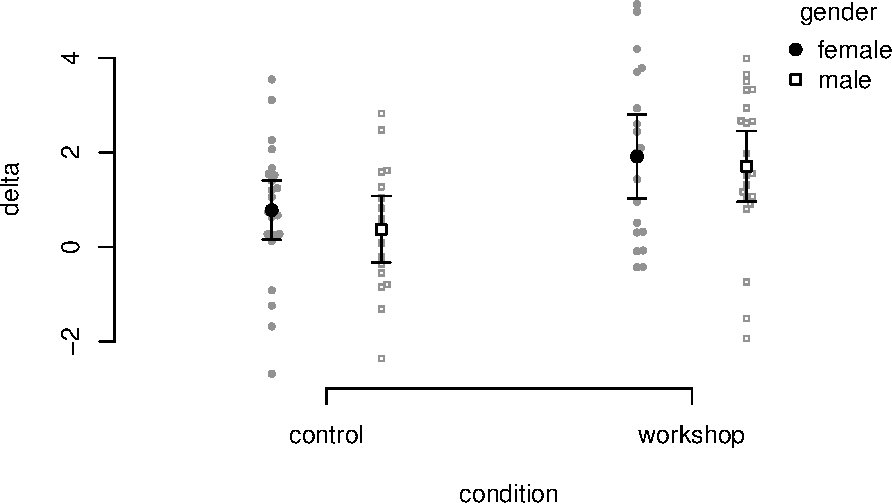
\includegraphics{manuscript_files/figure-latex/beeplot-1.pdf}

\hypertarget{regression}{%
\subsubsection{Regression}\label{regression}}

\begin{verbatim}
## Warning: 'data_findcols()' is deprecated and will be removed in a future update.
##   Its usage is discouraged. Please use 'data_find()' instead.

## Warning: 'data_findcols()' is deprecated and will be removed in a future update.
##   Its usage is discouraged. Please use 'data_find()' instead.

## Warning: 'data_findcols()' is deprecated and will be removed in a future update.
##   Its usage is discouraged. Please use 'data_find()' instead.
\end{verbatim}

We fitted a linear model (estimated using OLS) to predict delta with condition and conscientiousness (formula: delta \textasciitilde{} condition + conscientiousness). The model explains a statistically significant and moderate proportion of variance (R2 = 0.13, F(2, 77) = 5.79, p = 0.005, adj. R2 = 0.11). The model's intercept, corresponding to condition = control and conscientiousness = 0, is at 0.38 (95\% CI {[}-1.48, 2.24{]}, t(77) = 0.41, p = 0.687). Within this model:

\begin{itemize}
\tightlist
\item
  The effect of condition {[}workshop{]} is statistically significant and positive (beta = 1.21, 95\% CI {[}0.50, 1.93{]}, t(77) = 3.40, p = 0.001; Std. beta = 0.72, 95\% CI {[}0.30, 1.15{]})
\item
  The effect of conscientiousness is statistically non-significant and positive (beta = 0.04, 95\% CI {[}-0.30, 0.39{]}, t(77) = 0.25, p = 0.802; Std. beta = 0.03, 95\% CI {[}-0.19, 0.24{]})
\end{itemize}

Standardized parameters were obtained by fitting the model on a standardized version of the dataset. 95\% Confidence Intervals (CIs) and p-values were computed using the Wald approximation.

\begin{table}[tbp]

\begin{center}
\begin{threeparttable}

\caption{\label{tab:regression-table}Results from regression model.}

\begin{tabular}{llllll}
\toprule
Predictor & \multicolumn{1}{c}{$b$} & \multicolumn{1}{c}{95\% CI} & \multicolumn{1}{c}{$t$} & \multicolumn{1}{c}{$\mathit{df}$} & \multicolumn{1}{c}{$p$}\\
\midrule
Intercept & 0.38 & {}[-1.48, 2.24] & 0.41 & 77 & .687\\
Conditionworkshop & 1.21 & {}[0.50, 1.93] & 3.40 & 77 & .001\\
Conscientiousness & 0.04 & {}[-0.30, 0.39] & 0.25 & 77 & .802\\
\bottomrule
\end{tabular}

\end{threeparttable}
\end{center}

\end{table}

\hypertarget{discussion}{%
\section{Discussion}\label{discussion}}

An added benefit of rmarkdown and papaja is that you can simulate your data prior to data collection and already prepare your script with analyses.

\newpage

\hypertarget{references}{%
\section{References}\label{references}}

\begingroup
\setlength{\parindent}{-0.5in}
\setlength{\leftskip}{0.5in}

\hypertarget{refs}{}
\begin{CSLReferences}{1}{0}
\leavevmode\vadjust pre{\hypertarget{ref-alston2021}{}}%
Alston, J. M., \& Rick, J. A. (2021). A {Beginner}'s {Guide} to {Conducting Reproducible Research}. \emph{The Bulletin of the Ecological Society of America}, \emph{102}(2), e01801. \url{https://doi.org/10.1002/bes2.1801}

\leavevmode\vadjust pre{\hypertarget{ref-R-papaja}{}}%
Aust, F., \& Barth, M. (2020). \emph{{papaja}: {Create} {APA} manuscripts with {R Markdown}}. Retrieved from \url{https://github.com/crsh/papaja}

\leavevmode\vadjust pre{\hypertarget{ref-R-tinylabels}{}}%
Barth, M. (2022). \emph{{tinylabels}: Lightweight variable labels}. Retrieved from \url{https://cran.r-project.org/package=tinylabels}

\leavevmode\vadjust pre{\hypertarget{ref-R-lme4}{}}%
Bates, D., Mächler, M., Bolker, B., \& Walker, S. (2015). Fitting linear mixed-effects models using {lme4}. \emph{Journal of Statistical Software}, \emph{67}(1), 1--48. \url{https://doi.org/10.18637/jss.v067.i01}

\leavevmode\vadjust pre{\hypertarget{ref-R-Matrix}{}}%
Bates, D., \& Maechler, M. (2021). \emph{Matrix: Sparse and dense matrix classes and methods}. Retrieved from \url{https://CRAN.R-project.org/package=Matrix}

\leavevmode\vadjust pre{\hypertarget{ref-cruwell2019}{}}%
Crüwell, S., van Doorn, J., Etz, A., Makel, M., Moshontz, H., Niebaum, J., \ldots{} Schulte-Mecklenbeck, M. (2019). 8 {Easy Steps} to {Open Science}: {An Annotated Reading List}. \emph{ArXiv}. \url{https://doi.org/10.31234/osf.io/cfzyx}

\leavevmode\vadjust pre{\hypertarget{ref-R-purrr}{}}%
Henry, L., \& Wickham, H. (2020). \emph{Purrr: Functional programming tools}. Retrieved from \url{https://CRAN.R-project.org/package=purrr}

\leavevmode\vadjust pre{\hypertarget{ref-lindsay2018}{}}%
Lindsay, B. A. N. and D. S. (2018). Preregistration {Becoming} the {Norm} in {Psychological Science}. \emph{APS Observer}, \emph{31}. Retrieved from \url{https://www.psychologicalscience.org/observer/preregistration-becoming-the-norm-in-psychological-science}

\leavevmode\vadjust pre{\hypertarget{ref-R-report}{}}%
Makowski, D., Ben-Shachar, M. S., Patil, I., \& Lüdecke, D. (2021). Automated results reporting as a practical tool to improve reproducibility and methodological best practices adoption. \emph{CRAN}. Retrieved from \url{https://github.com/easystats/report}

\leavevmode\vadjust pre{\hypertarget{ref-R-tibble}{}}%
Müller, K., \& Wickham, H. (2021). \emph{Tibble: Simple data frames}. Retrieved from \url{https://CRAN.R-project.org/package=tibble}

\leavevmode\vadjust pre{\hypertarget{ref-R-base}{}}%
R Core Team. (2021). \emph{R: A language and environment for statistical computing}. Vienna, Austria: R Foundation for Statistical Computing. Retrieved from \url{https://www.R-project.org/}

\leavevmode\vadjust pre{\hypertarget{ref-R-afex}{}}%
Singmann, H., Bolker, B., Westfall, J., Aust, F., \& Ben-Shachar, M. S. (2022). \emph{Afex: Analysis of factorial experiments}. Retrieved from \url{https://CRAN.R-project.org/package=afex}

\leavevmode\vadjust pre{\hypertarget{ref-R-ggplot2}{}}%
Wickham, H. (2016). \emph{ggplot2: Elegant graphics for data analysis}. Springer-Verlag New York. Retrieved from \url{https://ggplot2.tidyverse.org}

\leavevmode\vadjust pre{\hypertarget{ref-R-stringr}{}}%
Wickham, H. (2019). \emph{Stringr: Simple, consistent wrappers for common string operations}. Retrieved from \url{https://CRAN.R-project.org/package=stringr}

\leavevmode\vadjust pre{\hypertarget{ref-R-forcats}{}}%
Wickham, H. (2021). \emph{Forcats: Tools for working with categorical variables (factors)}. Retrieved from \url{https://CRAN.R-project.org/package=forcats}

\leavevmode\vadjust pre{\hypertarget{ref-R-tidyverse}{}}%
Wickham, H., Averick, M., Bryan, J., Chang, W., McGowan, L. D., François, R., \ldots{} Yutani, H. (2019). Welcome to the {tidyverse}. \emph{Journal of Open Source Software}, \emph{4}(43), 1686. \url{https://doi.org/10.21105/joss.01686}

\leavevmode\vadjust pre{\hypertarget{ref-R-dplyr}{}}%
Wickham, H., François, R., Henry, L., \& Müller, K. (2022). \emph{Dplyr: A grammar of data manipulation}. Retrieved from \url{https://CRAN.R-project.org/package=dplyr}

\leavevmode\vadjust pre{\hypertarget{ref-R-tidyr}{}}%
Wickham, H., \& Girlich, M. (2022). \emph{Tidyr: Tidy messy data}. Retrieved from \url{https://CRAN.R-project.org/package=tidyr}

\leavevmode\vadjust pre{\hypertarget{ref-R-readr}{}}%
Wickham, H., Hester, J., \& Bryan, J. (2022). \emph{Readr: Read rectangular text data}. Retrieved from \url{https://CRAN.R-project.org/package=readr}

\leavevmode\vadjust pre{\hypertarget{ref-R-kableExtra}{}}%
Zhu, H. (2021). \emph{kableExtra: Construct complex table with 'kable' and pipe syntax}. Retrieved from \url{https://CRAN.R-project.org/package=kableExtra}

\end{CSLReferences}

\endgroup


\end{document}
